%Talk given virtually for SIAM UQ 2020 March
\documentclass[10pt,compress,xcolor={usenames,dvipsnames},aspectratio=169]{beamer}
%\documentclass[xcolor={usenames,dvipsnames},aspectratio=169]{beamer} %slides and 
%notes
\usepackage{amsmath,datetime,
	mathtools,
	bbm,
	%mathabx,
	array,
	booktabs,
	xspace,
	calc,
	colortbl,
 	graphicx}
\usepackage[usenames]{xcolor}
\usepackage[giveninits=false,backend=biber,style=nature, maxcitenames =10, mincitenames=9]{biblatex}
\addbibresource{FJHown23.bib}
\addbibresource{FJH23.bib}
\usepackage{newpxtext}
\usepackage[euler-digits,euler-hat-accent]{eulervm}
\usepackage{media9}
\usepackage[autolinebreaks]{mcode}
\usepackage[tikz]{mdframed}


\usetheme{FJHSlimNoFoot169}
\setlength{\parskip}{2ex}
\setlength{\arraycolsep}{0.5ex}

\DeclareMathOperator{\sol}{SOL}
\DeclareMathOperator{\app}{APP}
\DeclareMathOperator{\alg}{ALG}
\DeclareMathOperator{\ACQ}{ACQ}
\DeclareMathOperator{\ERR}{ERR}
\DeclareMathOperator{\COST}{COST}
\DeclareMathOperator{\COMP}{COMP}
\newcommand{\dataN}{\bigl(\hf(\vk_i)\bigr)_{i=1}^n}
\newcommand{\dataNj}{\bigl(\hf(\vk_i)\bigr)_{i=1}^{n_j}}
\newcommand{\dataNjd}{\bigl(\hf(\vk_i)\bigr)_{i=1}^{n_{j^\dagger}}}
\newcommand{\ERRN}{\ERR\bigl(\dataN,n\bigr)}

\newcommand{\Sapp}{S_{\textup{app}}}
\newcommand{\LambdaStd}{\Lambda^{\textup{std}}}
\newcommand{\LambdaSer}{\Lambda^{\textup{ser}}}
\newcommand{\LambdaAll}{\Lambda^{\textup{all}}}
\newcommand{\oton}{1\!:\!n}
\newcommand{\talert}[1]{\alert{\text{#1}}}
\DeclareMathOperator{\init}{init}
%\DeclareMathOperator{\app}{app}

\providecommand{\HickernellFJ}{H.}


\iffalse
The Successes and Challenges of Automatic Bayesian Cubature

The promise of Bayesian cubature is that with reasonable prior information (or assumptions) about the integrand, one can construct an optimal approximation to the corresponding (multidimensional) integral and simultaneously a credible interval.  Automatic Bayesian cubature uses increases the sample size until half-width of the credible interval is small enough.  We discuss how to choose appropriate covariance kernels, estimate their hyper-parameters, and construct the credible intervals, all with reasonable computational effort.  We also evaluate the performance of automatic Bayesian cubature on a variety of examples.


\fi

\renewcommand{\OffTitleLength}{-10ex}
\setlength{\FJHThankYouMessageOffset}{-8ex}
\title{The Successes and Challenges of Automatic Bayesian Cubature}
\author[]{Fred J. Hickernell}
\institute{Department of Applied Mathematics \\
	Center for Interdisciplinary Scientific Computation \\  Illinois Institute of Technology \\
	\href{mailto:hickernell@iit.edu}{\url{hickernell@iit.edu}} \quad
	\href{http://mypages.iit.edu/~hickernell}{\url{mypages.iit.edu/~hickernell}}}

\thanksnote{with Jagadeeswaran R. and the GAIL team \\
	partially supported by  NSF-DMS-1522687 and NSF-DMS-1638521 (SAMSI) \\[2ex]
	Thanks to the special session organizers
	
}
\event{SIAM-UQ 2020}
\date[]{March 2020}

\input FJHDef.tex


\newlength{\figwidth}
\setlength{\figwidth}{0.25\textwidth}

\newlength{\figwidthSmall}
\setlength{\figwidthSmall}{0.2\textwidth}

\newcommand{\financePict}{\href{http://i2.cdn.turner.com/money/dam/assets/130611131918-chicago-board-options-exchange-1024x576.jpg}{\includegraphics[width
		= 3cm]{ProgramsImages/130611131918-chicago-board-options-exchange-1024x576.jpg}}}
	
	\newcommand{\scoop}[1]{\parbox{#1}{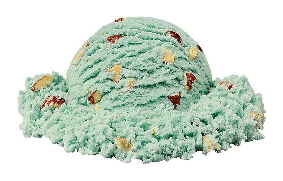
\includegraphics[width=#1]{IceCreamScoop.eps}}\xspace}
	\newcommand{\smallscoop}{\scoop{1cm}}
	\newcommand{\medscoop}{\scoop{1.8cm}}
	\newcommand{\largescoop}{\scoop{3cm}}
	\newcommand{\ICcone}[1]{\parbox{#1}{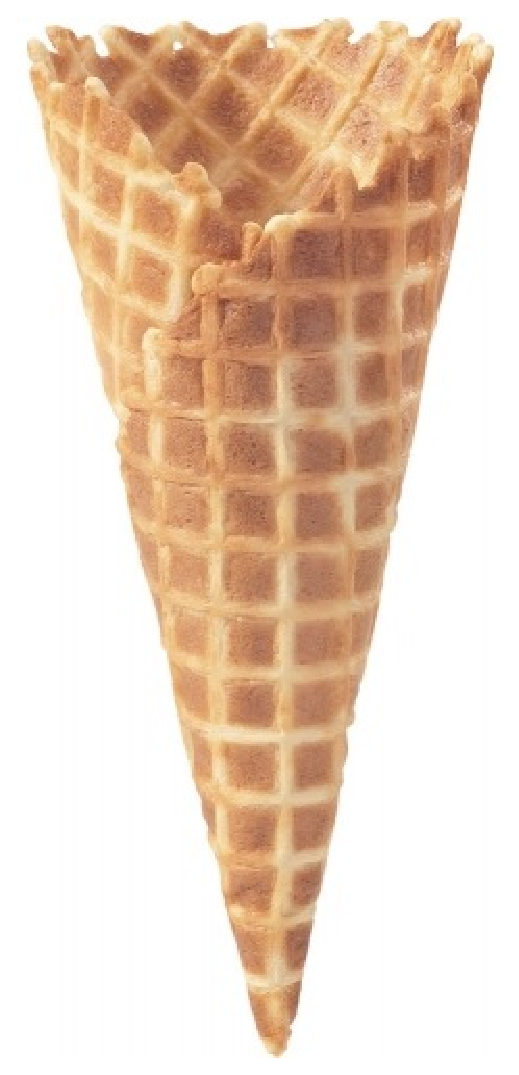
\includegraphics[width=#1,angle=270]{MediumWaffleCone.eps}}\xspace}
	\newcommand{\medcone}{\ICcone{1.2cm}}
	\newcommand{\largercone}{\parbox{2.2cm}{\vspace*{-0.2cm}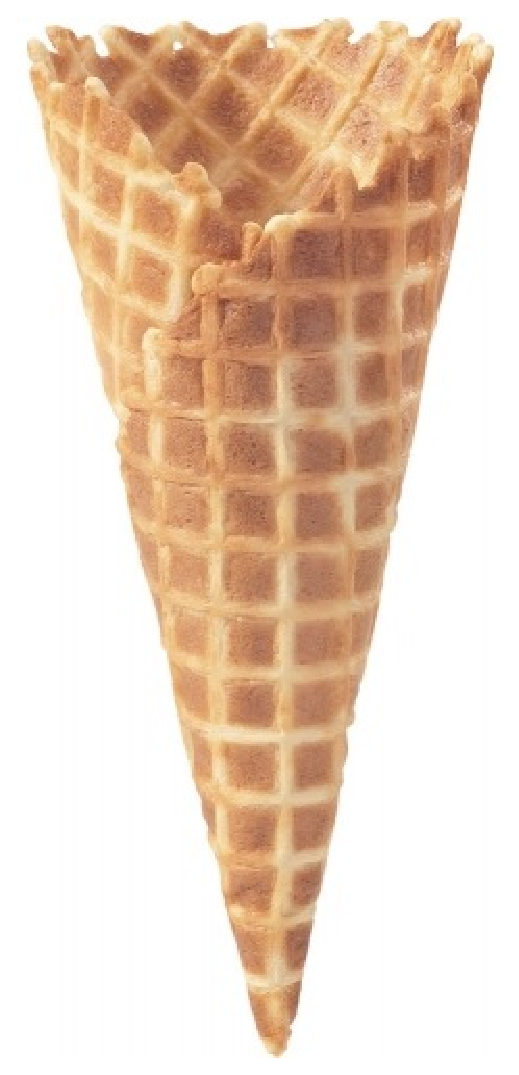
\includegraphics[width=1cm,angle=270]{MediumWaffleCone.eps}}\xspace}
	\newcommand{\largecone}{\ICcone{1.8cm}}
	\newcommand{\smallcone}{\parbox{1.1cm}{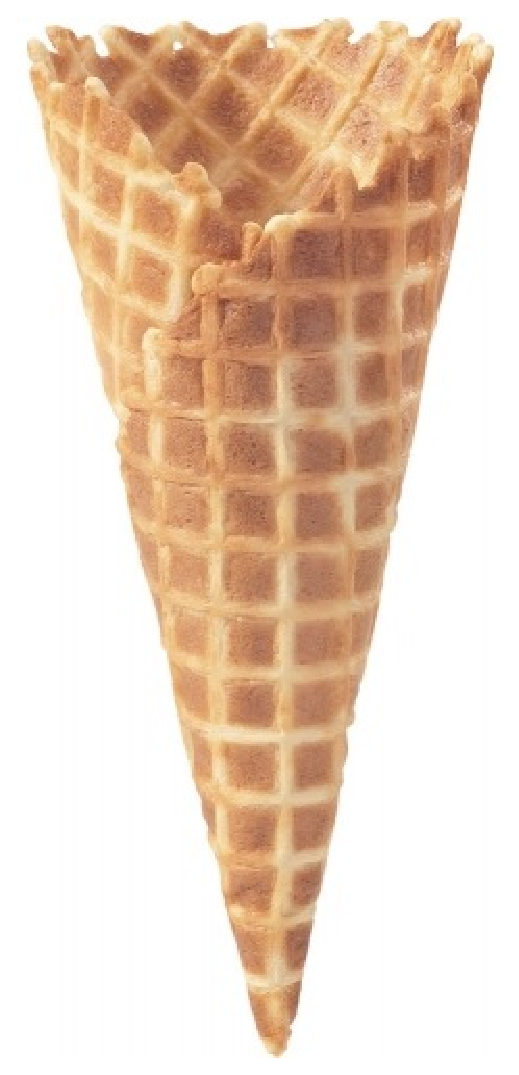
\includegraphics[width=0.5cm,angle=270]{MediumWaffleCone.eps}}\xspace}

	

\newcommand{\northeaststuff}[3]{
	\begin{tikzpicture}[remember picture, overlay]
	\node [shift={(-#1 cm,-#2 cm)}]  at (current page.north east){#3};
	\end{tikzpicture}}


\begin{document}
	\tikzstyle{every picture}+=[remember picture]
	\everymath{\displaystyle}

\frame{\titlepage}


\section{Introduction}

\begin{frame}
	{The Guaranteed Automatic Integration Library (GAIL) and QMCPy Teams}
	
	\vspace{-2ex}
	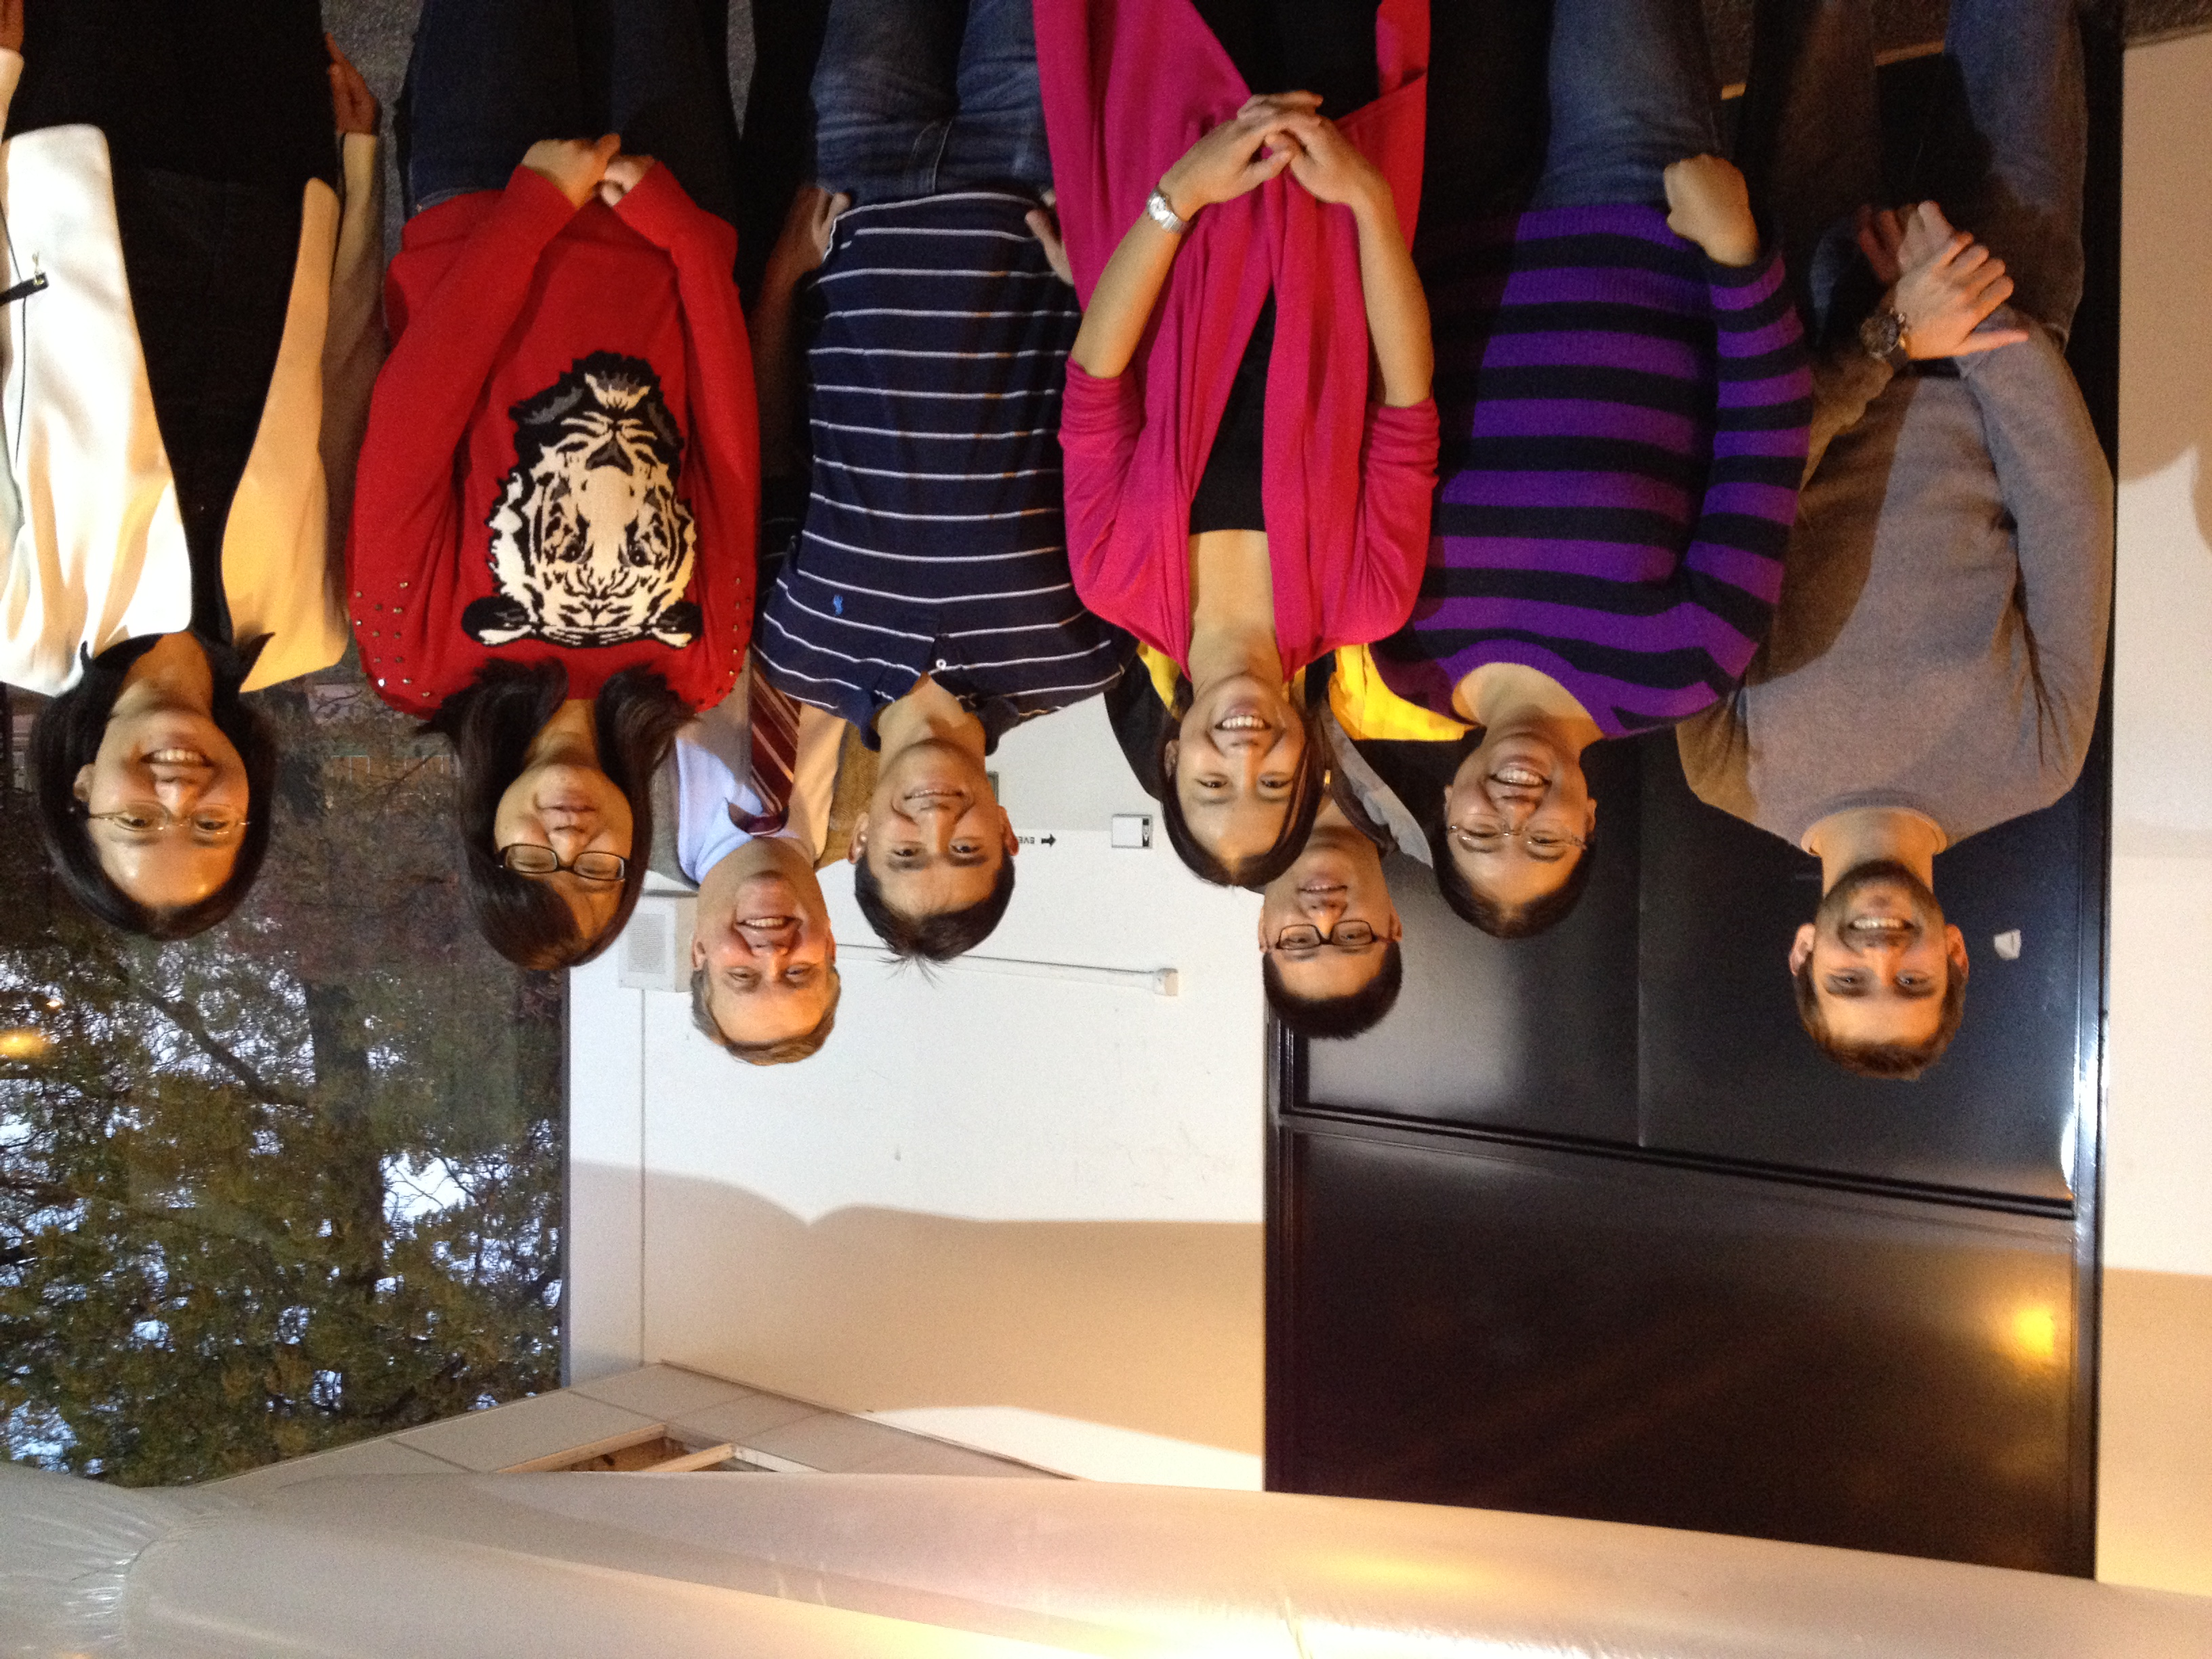
\includegraphics[angle = 180, origin = c, width = 0.32\textwidth]{ProgramsImages/GAIL2014RE.jpeg} \
	
\includegraphics[width = 0.32\textwidth]{ProgramsImages/GAILatSIAM2018Hi.jpeg} \ 
	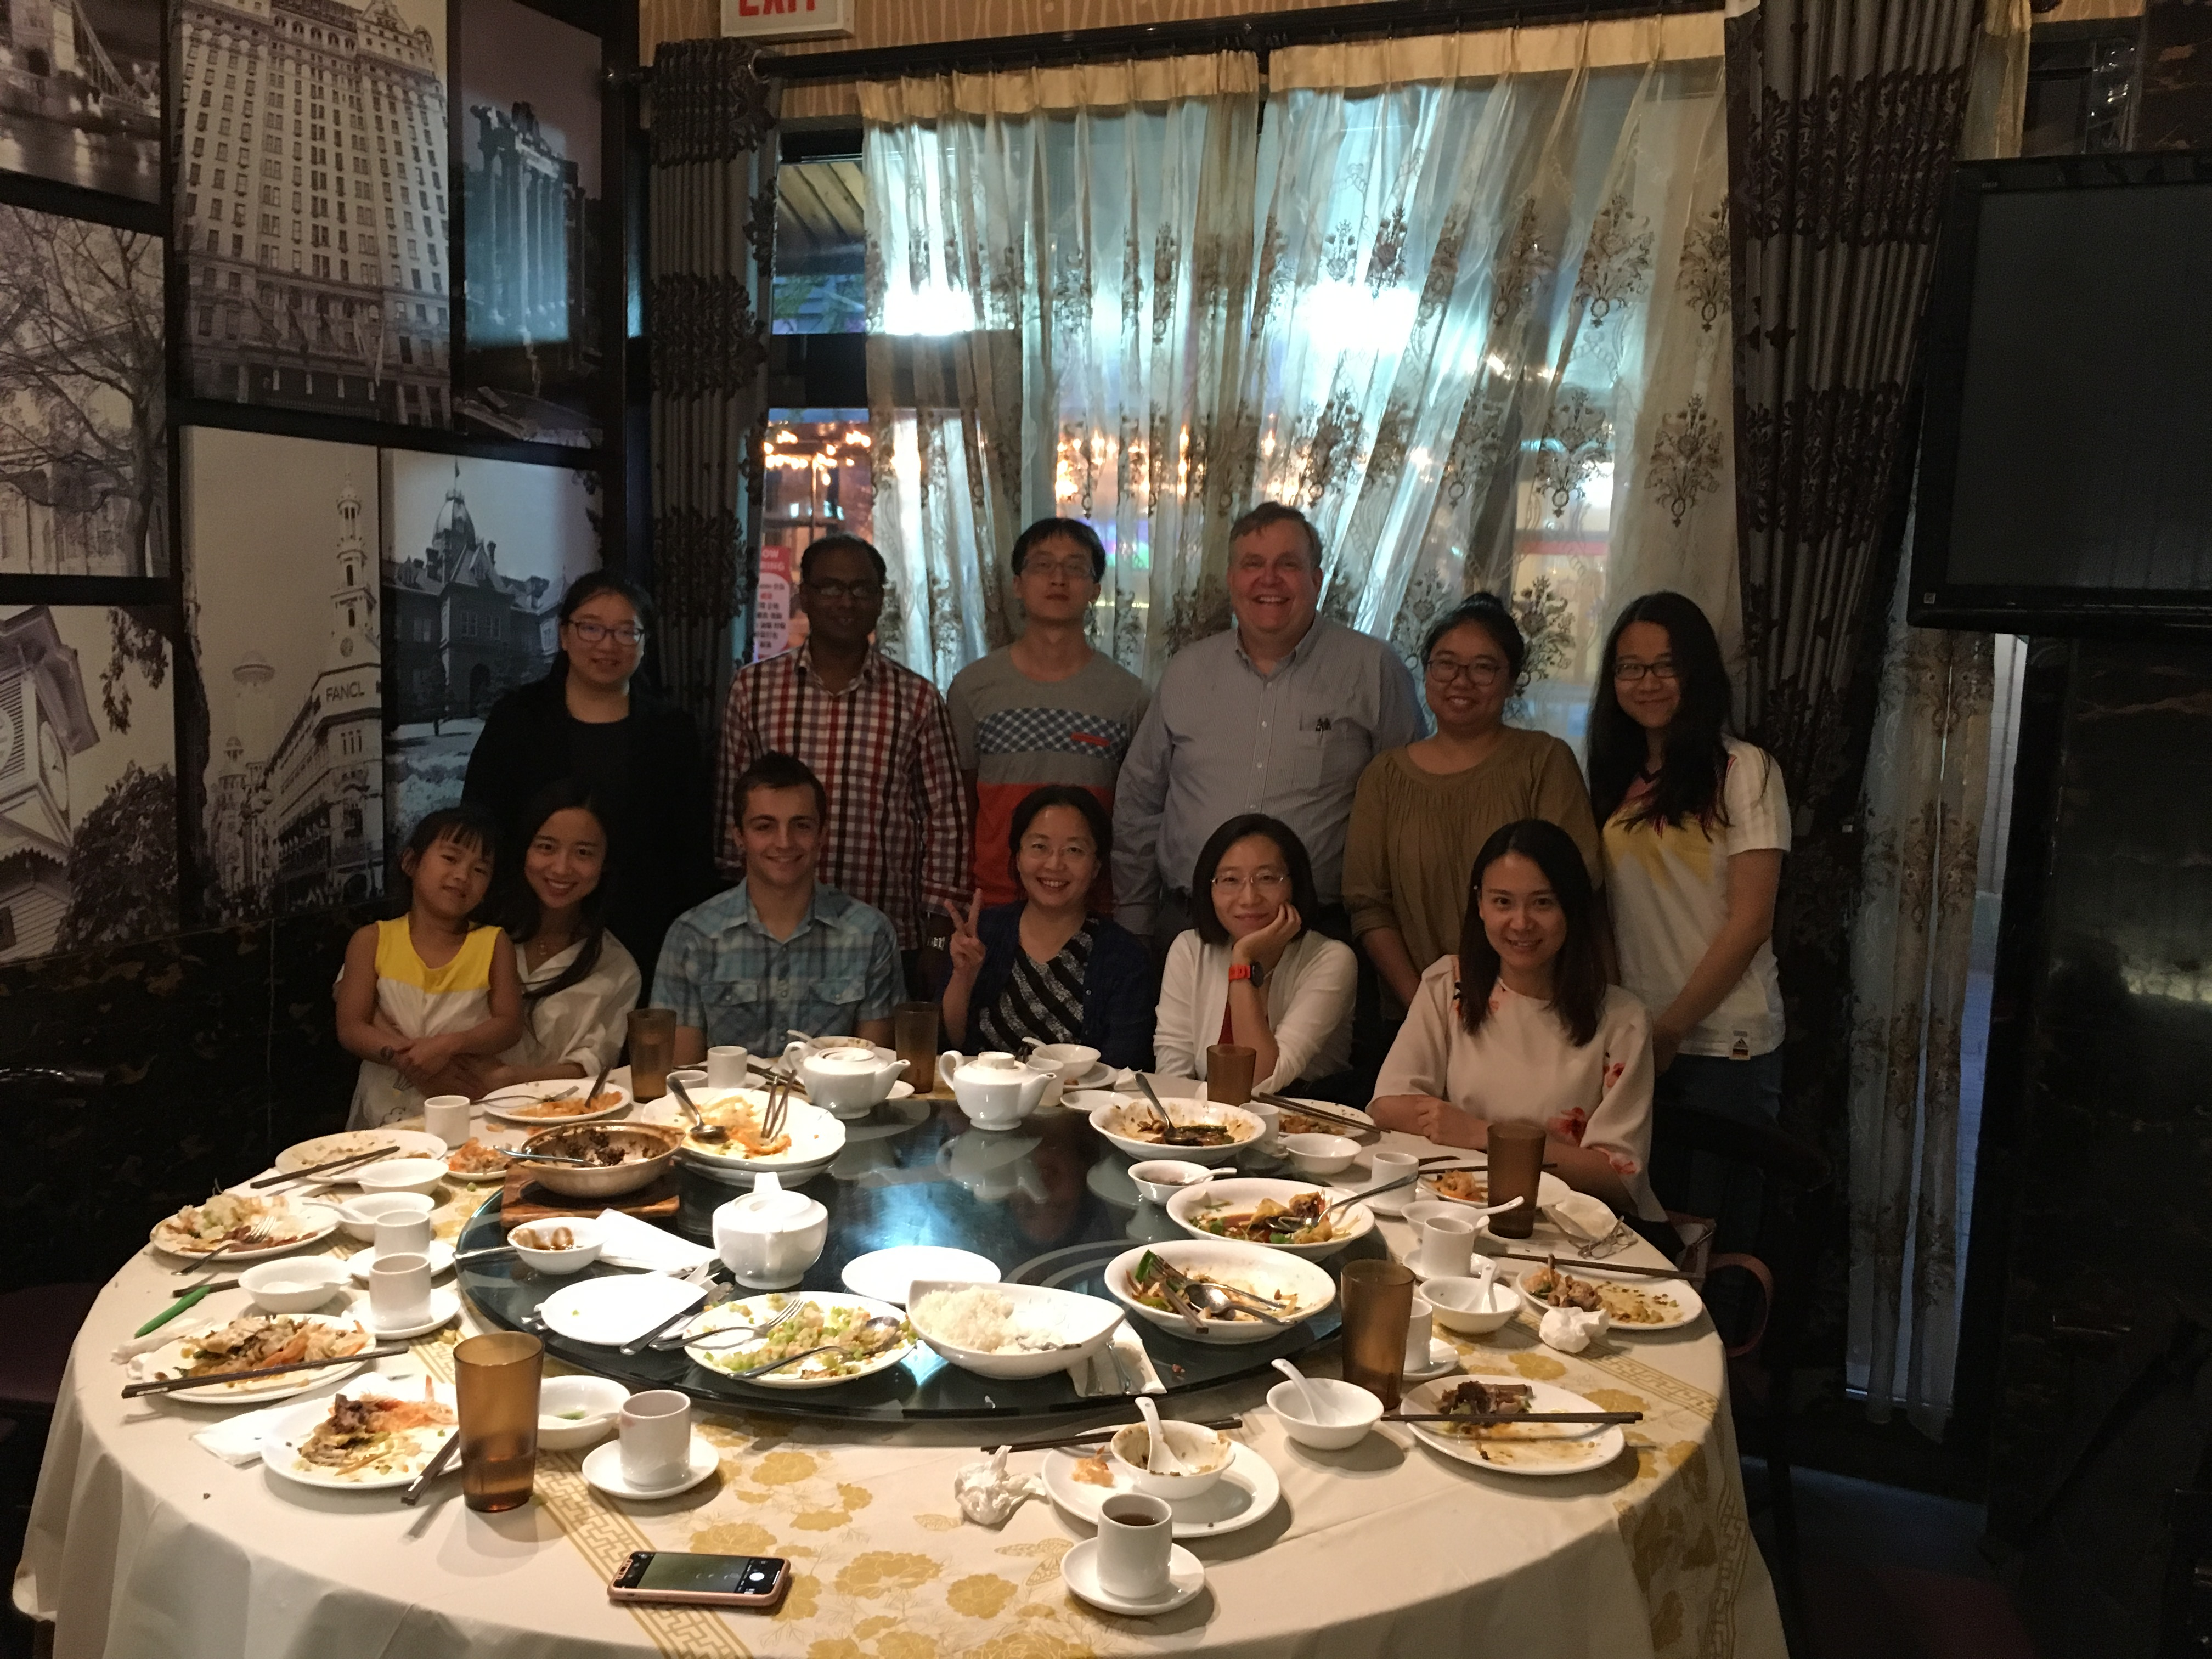
\includegraphics[width = 0.32\textwidth]{ProgramsImages/GAILatChinatown2018.jpg}
	
	\vspace{-3ex}
	\begin{tabular}{p{0.55\textwidth}p{0.42\textwidth}}
		
			
		\begin{itemize}
			\item Sou-Cheng Choi (Chief Data Scientist, Kamakura)
			
			\item Yuhan Ding (IIT PhD '15, Lecturer, IIT)
			
			\item Lan Jiang  (IIT PhD '16, Compass)
			
			\item Llu\'is Antoni Jim\'enez Rugama (IIT PhD '17, UBS)
			
			\item Jagadeeswaran Rathinavel (IIT PhD '19, Wi-Tronix)
			
			\item Aleksei Sorokin (IIT BS + MAS '21 exp.)
	
			
		\end{itemize}
	
	&
	
		\begin{itemize}
	
	
	\item Tong Xin (IIT MS, UIC PhD '20 exp.)
	
	\item Kan Zhang (IIT PhD '20 exp.)
	
	\item Yizhi Zhang (IIT PhD '18, Jamran Int'l)
	
	\item Xuan Zhou (IIT PhD '15, JP Morgan)
	
	\item and others
	
	
\end{itemize}

Adaptive software libraries \href{https://gailgithub.github.io/GAIL_Dev/}{\beamerbutton{GAIL}} and \href{https://qmcsoftware.github.io/QMCSoftware/}{\beamerbutton{QMCPy}}

	
	\end{tabular}
\end{frame}


\begin{frame}{Problem}

\vspace{-5ex}
\begin{itemize}
    \item Given \alert{black-box} function routine $f \colon \cx \subseteq \reals^d \to \reals$, e.g., output of a computer simulation
    
    \item \alert{Expensive} cost of a function value, $\$(f)$
    
    \item Want \alert{fixed tolerance algorithm} $\alg: \cc \times (0,\infty) \to L^{\infty}(\cx)$ such that 
    \[
    \norm[\infty]{f - \alg(f,\varepsilon)} \le \varepsilon \qquad \forall f \in \cc \text{ \alert{candidate set}}
    \]
    \alert{cheap} cost of an $\alg(f,\varepsilon)$ value\only<1>{, e.g., spline}\uncover<2->{
    \begin{gather*}
        \text{\alert{design or node array} }\mX \in \cx^n \subseteq \reals^{n \times d}, \qquad \text{\alert{function data} }  \vy = f(\mX)\in \reals^n \\
        \vx_{n+1} = \argmax_{\vx \in \cx} \ACQ(\vx,\mX,\vy) \text{ \alert{acquisition function}} \\
        \norm[\infty]{f - \app(\mX,\vy)} \le \ERR(\mX,\vy) \text{ \alert{data-driven error bound}} \qquad \forall n \in \naturals, \quad f \in \cc \\
        n^* = \min \, \{ n \in \naturals \colon \ERR(\mX,\vy) \le \varepsilon \} \text{ \alert{stopping criterion}} \\
        \alg(f,\varepsilon) = \app(\mX,\vy) \text{ \alert{fixed budget approximation} for this } n^*
    \end{gather*}}
 \end{itemize}
 
 \vspace{-6ex}
 \uncover<3->{\alert{Adaptive} sample size, design, and fixed budget approximation \\
 Assumes that \alert{what you see is almost what you get}}
    
\end{frame}


\section{Univariate, Low Accuracy}

\begin{frame}{Linear Splines}
\northeaststuff{3.7}{2.2}{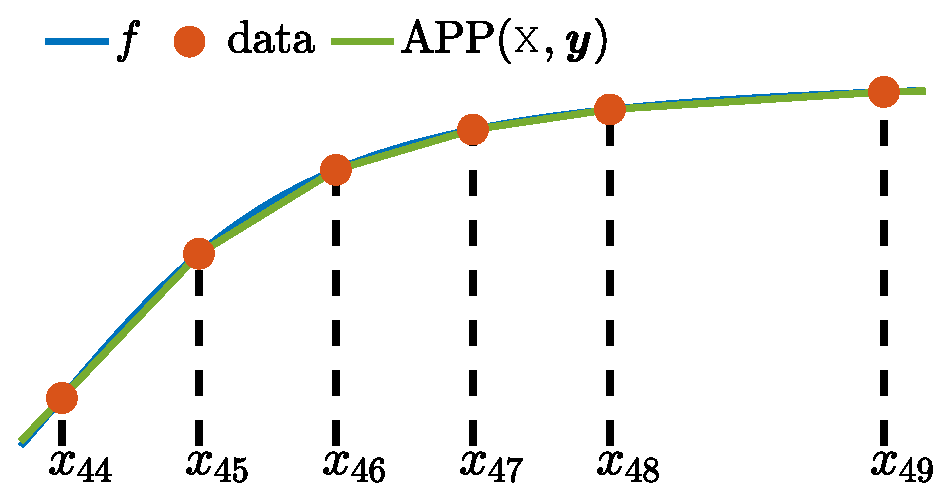
\includegraphics[width=6cm]{ProgramsImages/LinearSpline.eps}}

\vspace{-8ex}

\begin{minipage}{0.5\textwidth}
\vspace{-2ex}
    \begin{gather*}
    f  :[a,b] \to \reals \\
    a =: x_0 < x_1 < \cdots < x_n :=b, \quad \mX = \bigl( x_i \bigr)_{i=0}^n \talert{ data sites}\\ 
   \talert{function data } \vy = f(\mX)
\end{gather*}
\end{minipage}

\begin{gather*}
    \alert{\text{linear spline }}\app(\mX,\vy)  := \frac{x -x_i}{x_{i-1} - x_i} y_{i-1} +  \frac{x -x_{i-1}}{x_i - x_{i-1}} y_{i}, \quad x_{i-1} \le x \le x_i, \quad i \in \oton \\
    \norm[{\infty,[x_{i-1}, x_i]}]{f - \app(\mX,\vy)}  \le 
    \frac{(x_i - x_{i-1})^2\norm[{\infty,[x_{i-1},x_i]}]{f''}}{8}, \qquad i \in \oton, \quad  f \in \cw^{2,\infty}
\end{gather*}
\only<1-2>{\uncover<2>{Numerical analysis often stops here, leaving \alert{unanswered}  questions:

\vspace{-2ex}
\begin{itemize}
    \item How big should $n$ be to make $\norm[{\infty}]{f - \app(\mX,\vy)} \le \varepsilon$?
    \item How big is $\norm[{\infty,[x_{i-1},x_i]}]{f''}$?
    \item How best to choose $\mX$?
\end{itemize}
}}
    
\end{frame}


\begin{frame}{Linear Splines Error}
	\northeaststuff{3.7}{2.2}{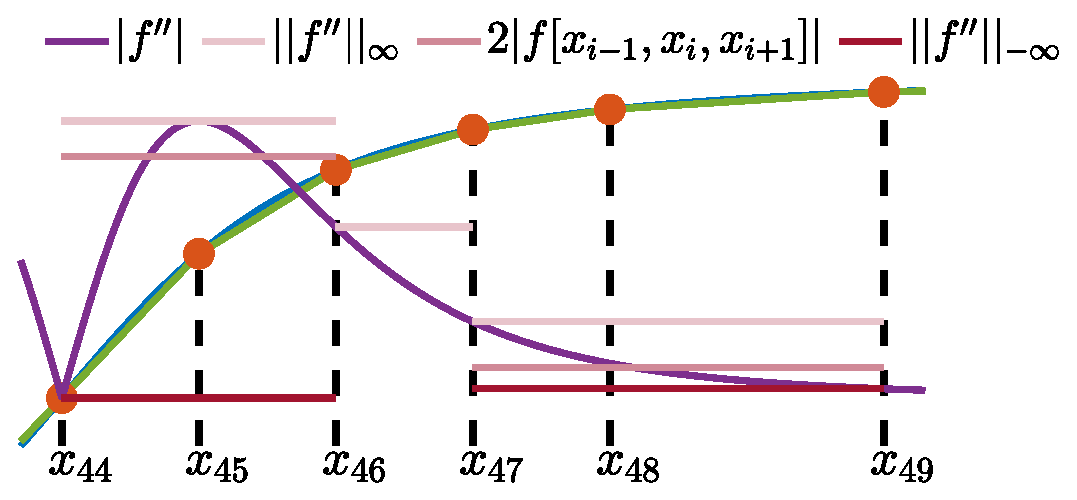
\includegraphics[width=6cm]{ProgramsImages/LinearSplineSecDeriv.eps}}
	
	\vspace{-8ex}
	
	\begin{minipage}{0.5\textwidth}
		\vspace{-2ex}
		\begin{gather*}
		f  :[a,b] \to \reals \\
		a =: x_0 < x_1 < \cdots < x_n :=b, \quad \mX = \bigl( x_i \bigr)_{i=0}^n \talert{ data sites}\\ 
		\talert{function data } \vy = f(\mX)
		\end{gather*}
	\end{minipage}
	
	\begin{gather*}
	\only<1-2>{\alert{\text{linear spline }}\app(\mX,\vy)  := \frac{x -x_i}{x_{i-1} - x_i} y_{i-1} +  \frac{x -x_{i-1}}{x_i - x_{i-1}} y_{i}, \quad x_{i-1} \le x \le x_i, \quad i \in \oton \\}
	\norm[{\infty,[x_{i-1}, x_i]}]{f - \app(\mX,\vy)}  \le 
	\frac{1}{8}(x_i - x_{i-1})^2\norm[{\infty,[x_{i-1},x_i]}]{f''}\only<1-2>{,}\only<3->{\le \max_{\pm} \ERR_{i,\pm}(\mX,\vy),} \quad i \in \oton, \;  f \in \only<1-2>{\cw^{2,\infty}}\only<3->{\cc}
   \only<1-2>{\\ \norm[{-\infty, [x_{i-1},x_{i+1}]}]{f''}
	\le \underbrace{\Biggl \lvert \frac{\frac{y_{i+1} - y_i}{x_{i+1} - x_i} - \frac{y_i - y_{i-1}}{x_i - x_{i-1}}}{(x_{i+1} - x_{i-1})/2}\Biggr \rvert}_{\substack{D_i(\mX,\vy) = 2\abs{f[x_{i-1},x_i,x_{i+1}]} \talert{ data based}\\ \talert{abs.\ $2^{\text{nd}}$ deriv.\ of interp.\ poly.}}}
	\le \norm[{\infty, [x_{i-1},x_{i+1}]}]{f''}}
	\end{gather*}
	\vspace{-3ex}
	\uncover<2->{\begin{multline*}
	\talert{candidate set }	\cc : =  \Bigl \{ f \in \cw^{2,\infty}  : \abs{f''(x)} \le \max \bigl (\fC(h_{-}) \abs{f''(x - h_-)},  \fC(h_{+})\abs{f''(x + h_+)} \bigr), \ 
	0 < h_{\pm} < \fh, \\[-1ex]
	a < x < b \Bigr\} \qquad
	\talert{inflation factor } \fC(h) := \frac{\fC_0 \fh}{\fh - h} \qquad \talert{$\abs{f''}$ does not change abruptly}
	\end{multline*}}

\only<3->{\vspace{-8ex} 
	\begin{gather*}
\ERR_{i,-}(\mX,\vy) =  \frac18 (x_i-x_{i-1})^2\fC(x_i - x_{i-3}) D_{i-2}(\mX,\vy), \\
\ERR_{i,+}(\mX,\vy) = \frac 18 (x_i-x_{i-1})^2\fC(x_{i+2} - x_{i-1}) D_{i+1}(\mX,\vy)\\
D_i(\mX,\vy) = 2\abs{f[x_{i-1},x_i,x_{i+1}]}  \talert{ data based, absolute\ $2^{\text{nd}}$ derivative\ of interpoplating\ polynomial}
\end{gather*}}
\end{frame}

\begin{frame}
	\frametitle{Adaptive Linear Spline Algorithm\footfullcite{ChoEtal17a}}
	\only<1-2>{\northeaststuff{3.7}{2.5}{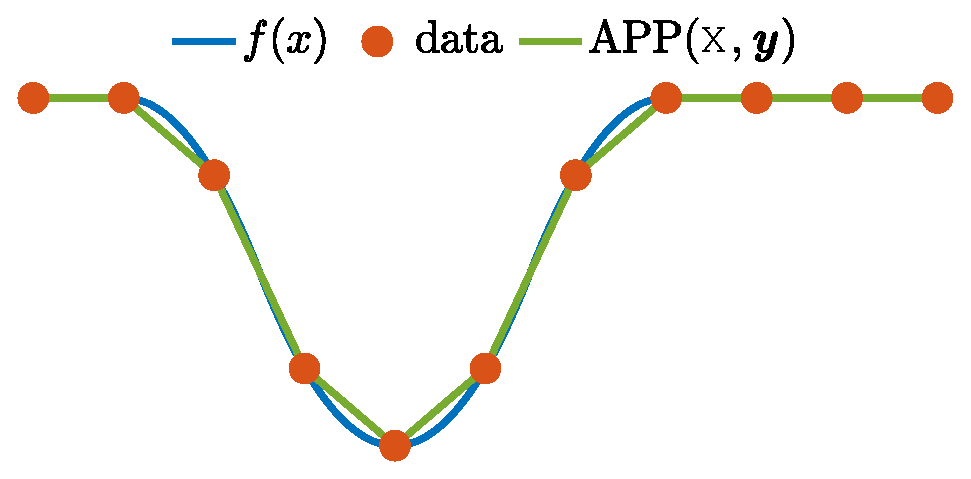
\includegraphics[width=6cm]{ProgramsImages/sampling-funappxg-1.eps}}}
	\only<3>{\northeaststuff{3.7}{2.5}{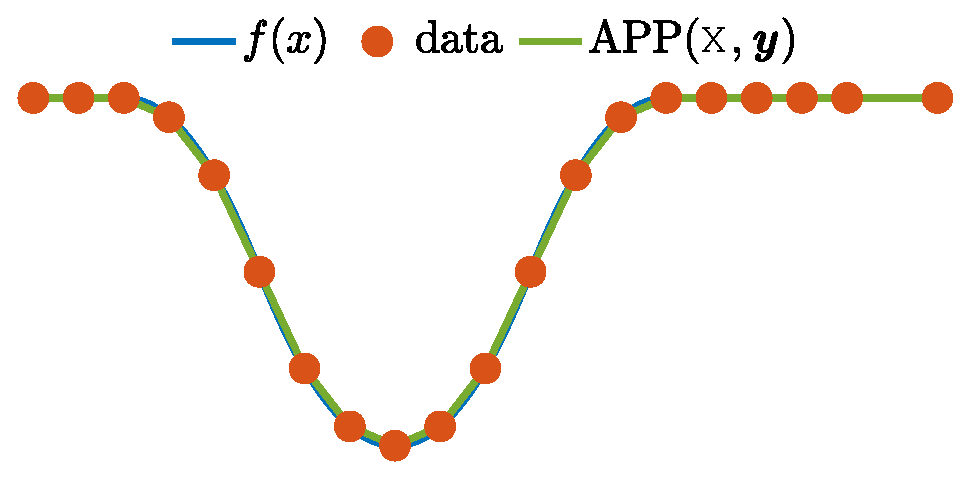
\includegraphics[width=6cm]{ProgramsImages/sampling-funappxg-2.eps}}}
	\only<4>{\northeaststuff{3.7}{2.5}{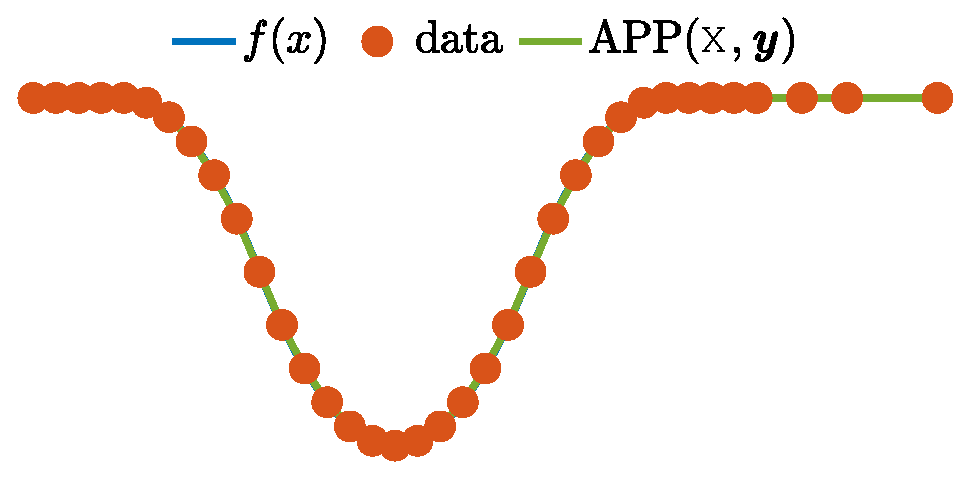
\includegraphics[width=6cm]{ProgramsImages/sampling-funappxg-3.eps}}}
	
	\vspace{-10ex}
	
	\parbox{4.2cm}{
		Given $n_{\init} \ge 4$, $\fC_0 \ge 1$: 
		
		\vspace{-3ex}
		
		\begin{gather*}
		\fh  = \left \lceil \frac{3(b-a)}{n_{\init}-1} \right \rceil , \qquad 
		\fC(h) = \frac{\fC_0 \fh}{\fh - h} \\
		n = n_{\init}, \qquad 
		x_i = a + i(b-a)/n
		\end{gather*}
	}
	
	
	\vspace{-2ex}
	
	\begin{description}
		\item<2->[Step 1.] Compute data based $\ERR_{i,\pm}(\mX,\vy)$ for $i = 1, \ldots, n$.
		\item<2->[Step 2.] Construct $\ci$, the index set of subintervals that might be split:
		\begin{equation*}
		\ci = \bigl\{i \in 1\! :\! n \ : \ \ERR_{i\pm j,\mp}(\mX,\vy) > \varepsilon, \ j = 0, 1, 2\}
		\end{equation*}
		\item<3->[Step 3.]  If $\ci = \emptyset$, return $\alg(f,\varepsilon) = \app(\mX,\vy)$ as the approximation satisfying the error tolerance.  Otherwise split those intervals in $\ci$ with largest width and go to Step 1 (\alert{acquisition function}). 
	\end{description}
	
\end{frame}


\begin{frame}
	\frametitle{Highlights of Adaptive Linear Spline Algorithm\footfullcite{ChoEtal17a}}
	\only<1,4,7>{\northeaststuff{3.7}{3}{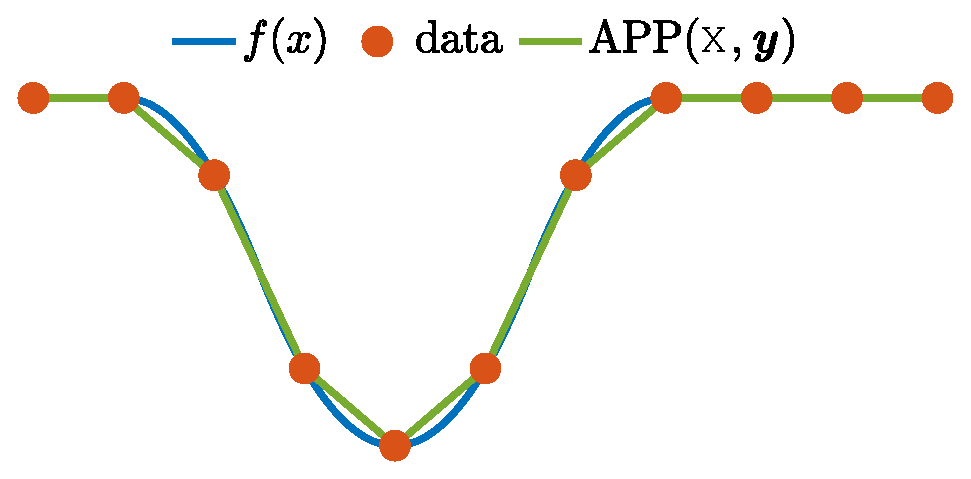
\includegraphics[width=6cm]{ProgramsImages/sampling-funappxg-1.eps}}}
	\only<2,5,8>{\northeaststuff{3.7}{3}{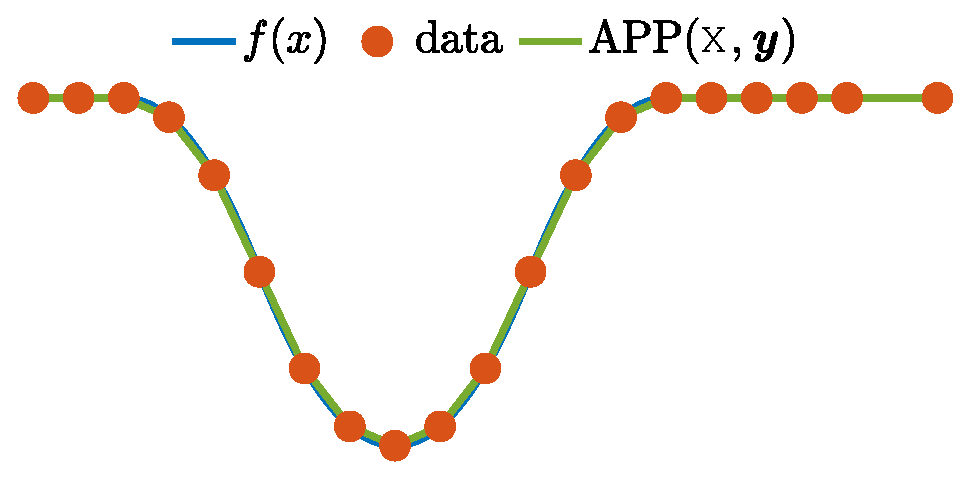
\includegraphics[width=6cm]{ProgramsImages/sampling-funappxg-2.eps}}}
	\only<3,6,9->{\northeaststuff{3.7}{3}{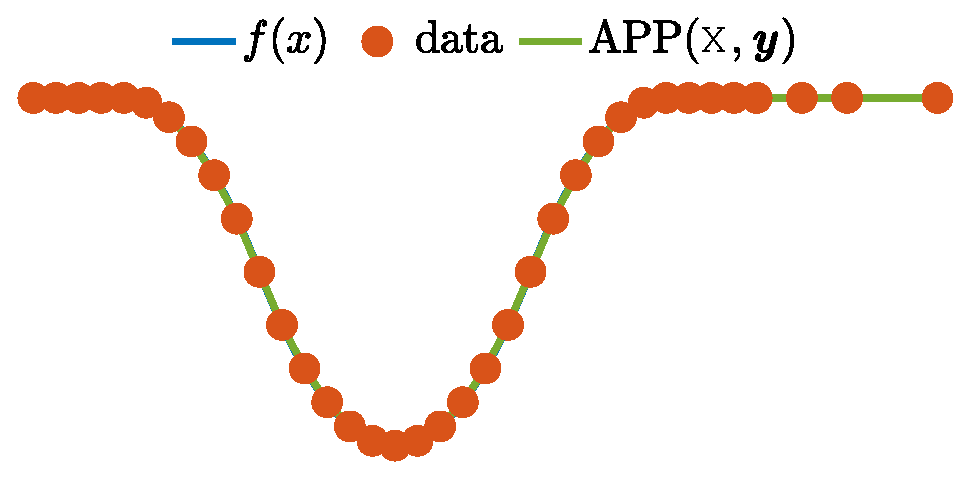
\includegraphics[width=6cm]{ProgramsImages/sampling-funappxg-3.eps}}}
	
	\vspace{-10ex}
	

\begin{itemize}[<+->]
	\item Defined for \alert{cone candidate set, $\cc$}, whose definition \\
	does not depend on the algorithm
	
	\item \alert{Guaranteed} to succeed for all $f \in \cc$

	\item Candidate set $\cc$ \alert{excludes spikes}, \\
	i.e., two nearby inflection points
	
	\item $\cc$ formalizes \alert{what you see is almost what you get}

	\item \alert{Impossible} to have an algorithm for all $f \in \cw^{2,\infty}$ \\
	since $\cw^{2,\infty}$ contains arbitrarily  large functions that look like $0$
	
	\item Adaptive algorithms \alert{do not help for ball} candidate sets 
	$\cc = \{ f : \norm[\infty]{f''} \le R\}$
	
	\item $\cost(\alg,f,\varepsilon,\cc) \asymp \sqrt{\frac{\fC_0 \norm[\alert{\frac 12}]{f''}}{\varepsilon}} \asymp \comp(f,\varepsilon,\cc)$ \alert{ optimal}
	
	\item Does not allow for  \alert{smoothness} to be inferred
	
	\item Not \alert{multivariate}
	
\end{itemize}
	
\end{frame}

\section{Multivariate, Reproducing Kernel Hilbert Space}

\begin{frame}{Approximation via Reproducing Kernel Hilbert Spaces (RKHSs) \footfullcite{Fas07a,FasMcC15a}}
\northeaststuff{3.7}{3}{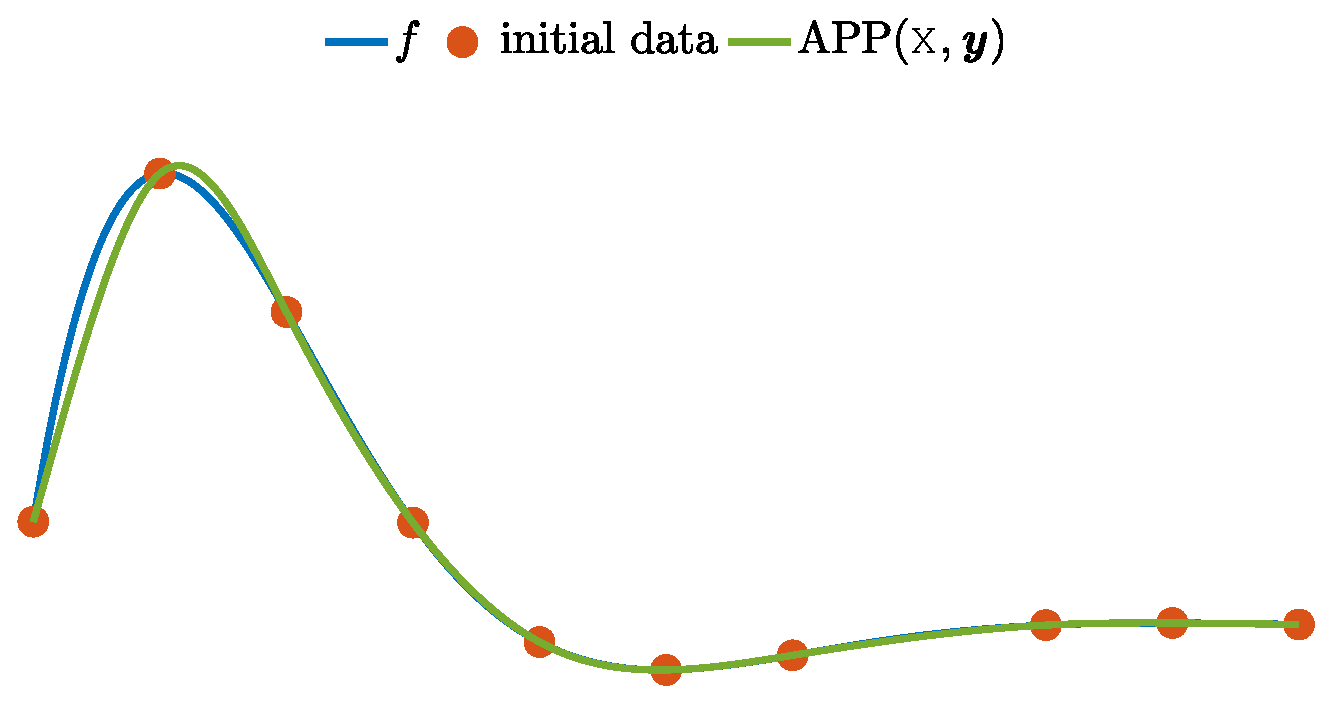
\includegraphics[width=6cm]{ProgramsImages/fandDataAndAppx.eps}}
	
		\vspace{-8ex}

\begin{minipage}{7cm}
$\cf$ is a \alert{Hilbert space }  with \alert{reproducing kernel} \\ $K : \cx \times \cx \to \reals$ 

\vspace{-4ex}
\begin{gather*}
K(\mX,\mX) \talert{ positive definite } \forall \mX \\
K(\cdot,\vx) \in \cf, \quad 
f(\vx) = \ip[\cf]{K(\cdot,\vx)}{f} \qquad \forall \vx \in \cx, \\
\text{e.g., } K(\vt,\vx) = (1 + \norm[2]{\vt - \vx}) \exp\bigl( -\norm[2] {\vt - \vx}\bigr) \talert{ Mat\'ern}
\end{gather*}
\end{minipage}

\vspace{-2ex}
\uncover<2->{Optimal (minimum norm) interpolant is 
\[
\app(\mX,\vy) = K(\cdot,\mX)\bigl(K(\mX,\mX) \bigr)^{-1} \vy, \qquad \vy = f(\mX)
\] 

\vspace{-6ex}
\begin{align*}
\norm[\infty]{f - \app(\mX,\vy)}^2  &\le \bignorm[\infty]{K(\cdot,\cdot) -  K(\cdot,\mX)\bigl(K(\mX,\mX) \bigr)^{-1} K(\mX, \cdot)} \ \norm[\cf]{f - \app(\mX,\vy)}^2 \quad \talert{known}\uncover<4->{\\
& \le \bignorm[\infty]{K(\cdot,\cdot) -  K(\cdot,\mX)\bigl(K(\mX,\mX) \bigr)^{-1} K(\mX, \cdot)} \ \frac{\fC^2(\mX)}{1 - \fC^2(\mX)} \ \norm[\cf]{ \app(\mX,\vy)}^2 =: \alert{\ERR^2(\mX,\vy)}}
\end{align*}
\vspace{-1ex}
\uncover<3->{\[
\talert{candidate set } \cc = \bigl\{ f \in \cf :  \norm[\cf]{f - \app(\mX,\vy)} \le  \alert{\fC(\mX)} \norm[\cf]{f} \bigr\}
\]}}

\end{frame}

\begin{frame}{Error and Acquisition for Optimal RKHS Approximation}
	\only<1>{\northeaststuff{3.7}{3}{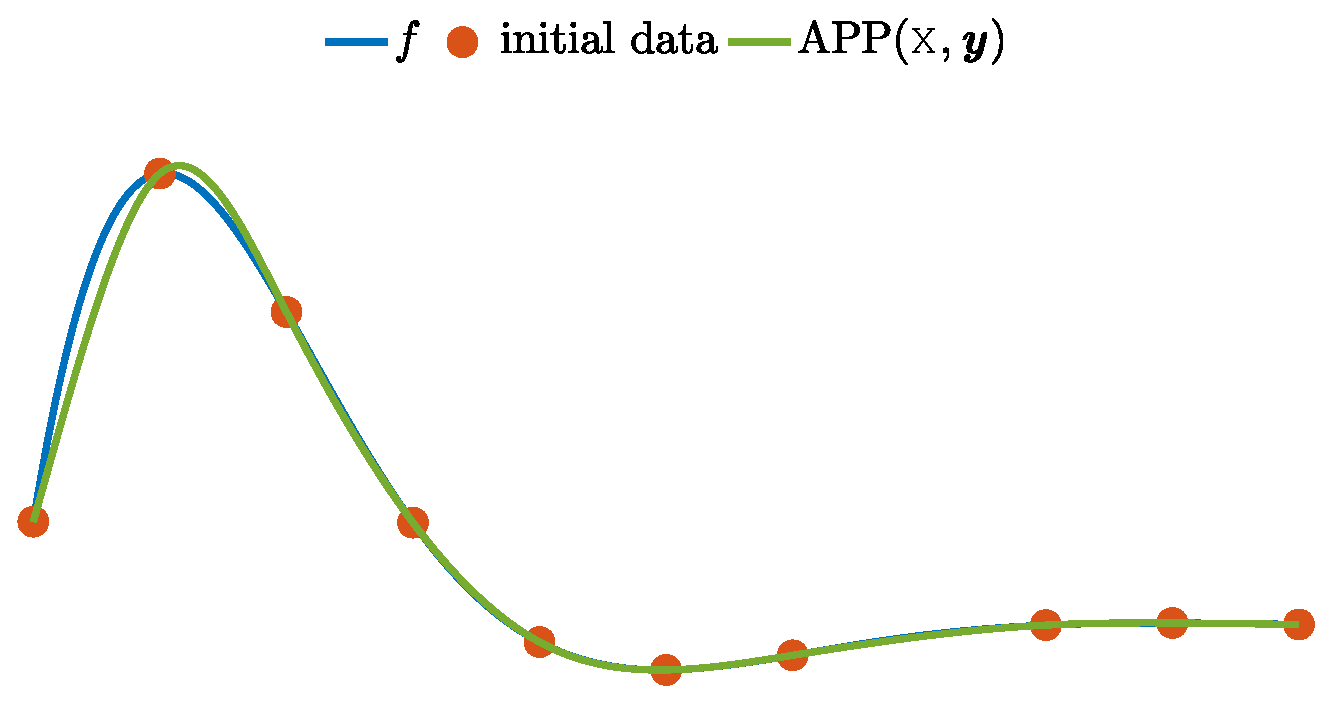
\includegraphics[width=6cm]{ProgramsImages/fandDataAndAppx.eps}}}
	\only<2>{\northeaststuff{3.7}{3}{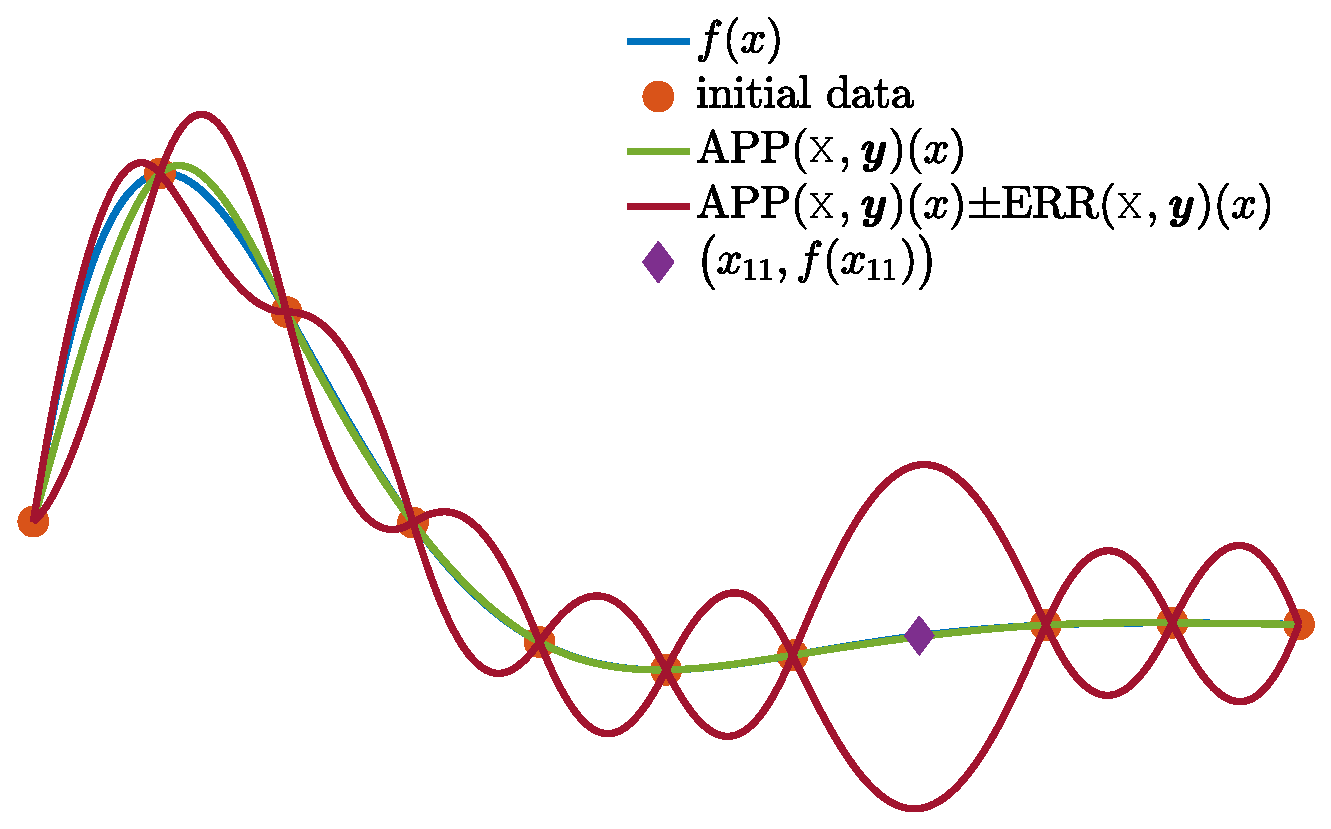
\includegraphics[width=6cm]{ProgramsImages/fandDataAndAppxAndRMSPE.eps}}}
	\vspace{-5ex}
	
	\begin{minipage}{7cm}
		$\cf$ is a \alert{Hilbert space }  with \alert{reproducing kernel} \\ $K : \cx \times \cx \to \reals$ 
		
		\vspace{-4ex}
		\begin{gather*}
		\text{e.g., } K(\vt,\vx) = (1 + \norm[2]{\vt - \vx}) \exp\bigl( -\norm[2] {\vt - \vx}\bigr) \talert{ Mat\'ern} \\
		\app(\mX,\vy) = K(\cdot,\mX)\bigl(K(\mX,\mX) \bigr)^{-1} \vy, \qquad \vy = f(\mX) \\
		\talert{candidate set } \cc = \bigl\{ f \in \cf :  \norm[\cf]{f - \app(\mX,\vy)} \le  \alert{\fC(\mX)} \norm[\cf]{f} \bigr\}
		\end{gather*}
	\end{minipage}
	
	\vspace{-2ex}
	\begin{align*}
	\norm[\infty]{f - \app(\mX,\vy)}^2  &\le \bignorm[\infty]{K(\cdot,\cdot) -  K(\cdot,\mX)\bigl(K(\mX,\mX) \bigr)^{-1} K(\mX, \cdot)} \ \norm[\cf]{f - \app(\mX,\vy)}^2 \quad \talert{known}\\
		& \le \bignorm[\infty]{K(\cdot,\cdot) -  K(\cdot,\mX)\bigl(K(\mX,\mX) \bigr)^{-1} K(\mX, \cdot)} \ \frac{\fC^2(\mX)}{1 - \fC^2(\mX)} \ \norm[\cf]{ \app(\mX,\vy)}^2 =: \alert{\ERR^2(\mX,\vy)} \\
	\ACQ(\vx,\mX,\vy)  & : = \bigl[K(\vx,\vx) -  K(\vx,\mX)\bigl(K(\mX,\mX) \bigr)^{-1} K(\mX, \vx) \bigr]  \ \frac{\fC^2(\mX)}{1 - \fC^2(\mX)}  \ \underbrace{\norm[\cf]{ \app(\mX,\vy)}^2}_{\alert{\vy^T(K(\mX,\mX) )^{-1} \vy}} \\[-1ex]
	        \vx_{n+1} &= \argmax_{\vx \in \cx} \ACQ(\vx,\mX,\vy) \text{ \alert{acquisition function}} \\
	\alg(f,\varepsilon) &= \app(\mX,\vy) \quad \text{for } n^* = \min \, \{ n \in \naturals \colon \ERR(\mX,\vy) \le \varepsilon \} \text{ \alert{stopping criterion}} 
	\end{align*}

\end{frame}

\begin{frame}{Must Infer Kernel from $\vy = f(\mX)$}
	\vspace{-2ex}
	\only<2>{\northeaststuff{3.5}{2.45}{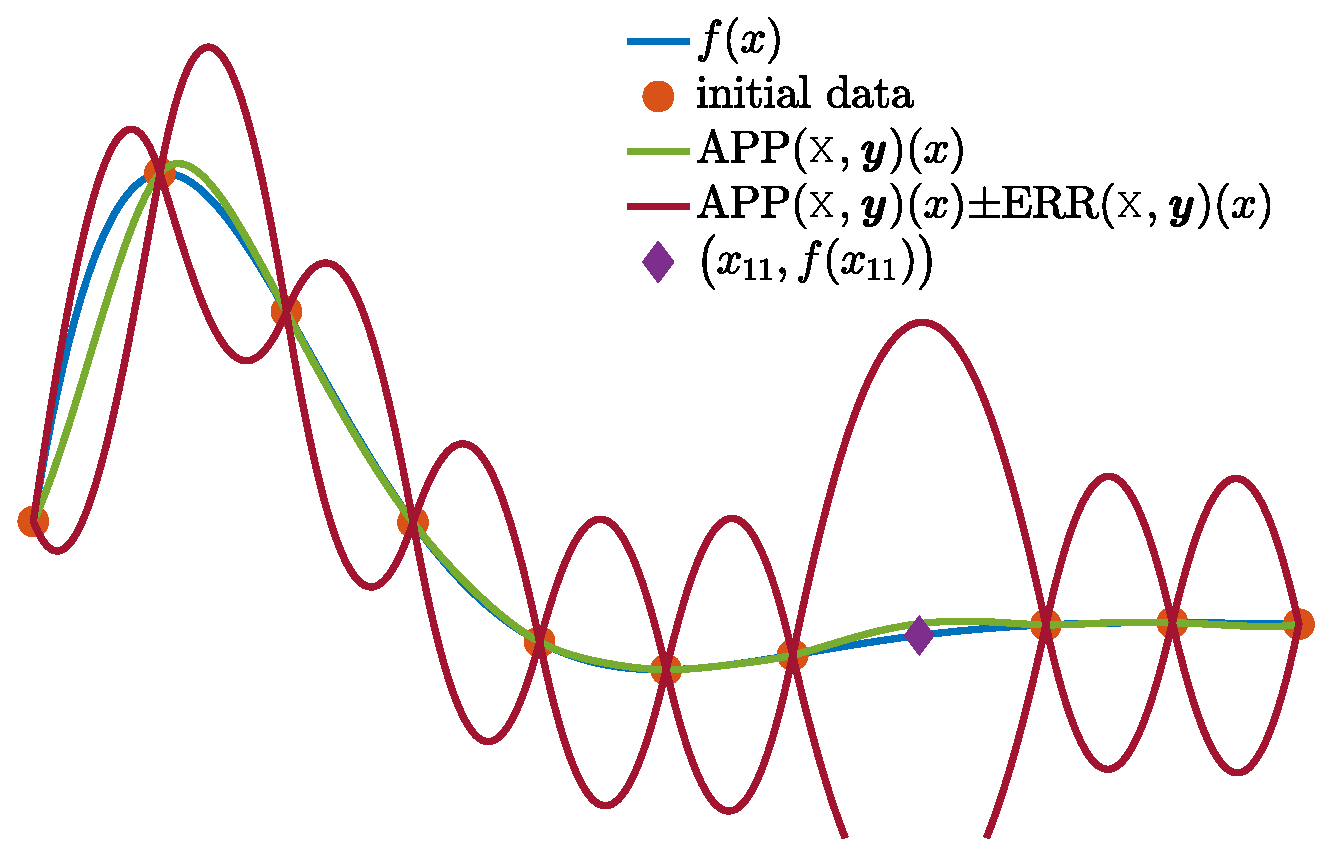
\includegraphics[width=6cm]{ProgramsImages/fandDataAndAppxAndRMSPEOpt.eps}}\vspace{-5ex}}
		\only<3>{\northeaststuff{3.5}{2.45}{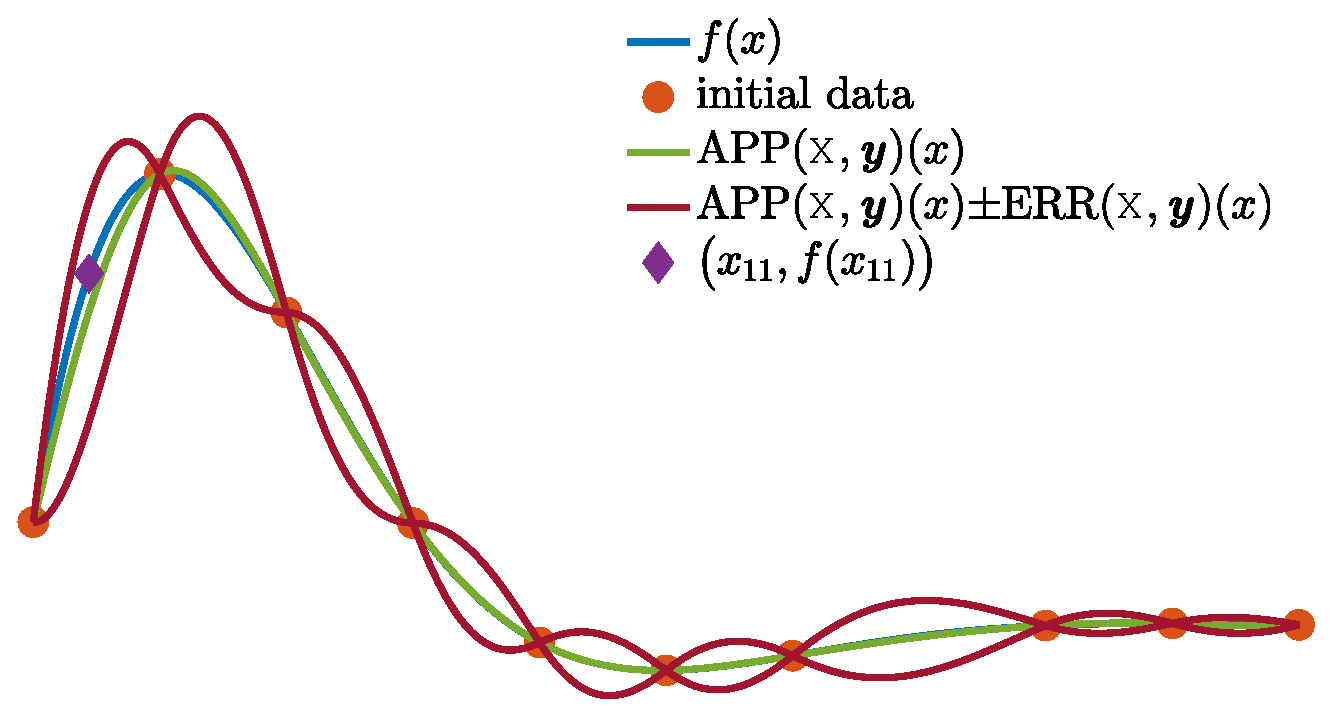
\includegraphics[width=6cm]{ProgramsImages/fandDataAndAppxAndRMSPEOpty.eps}}\vspace{-5ex}}
		\only<4>{\northeaststuff{3.5}{2.45}{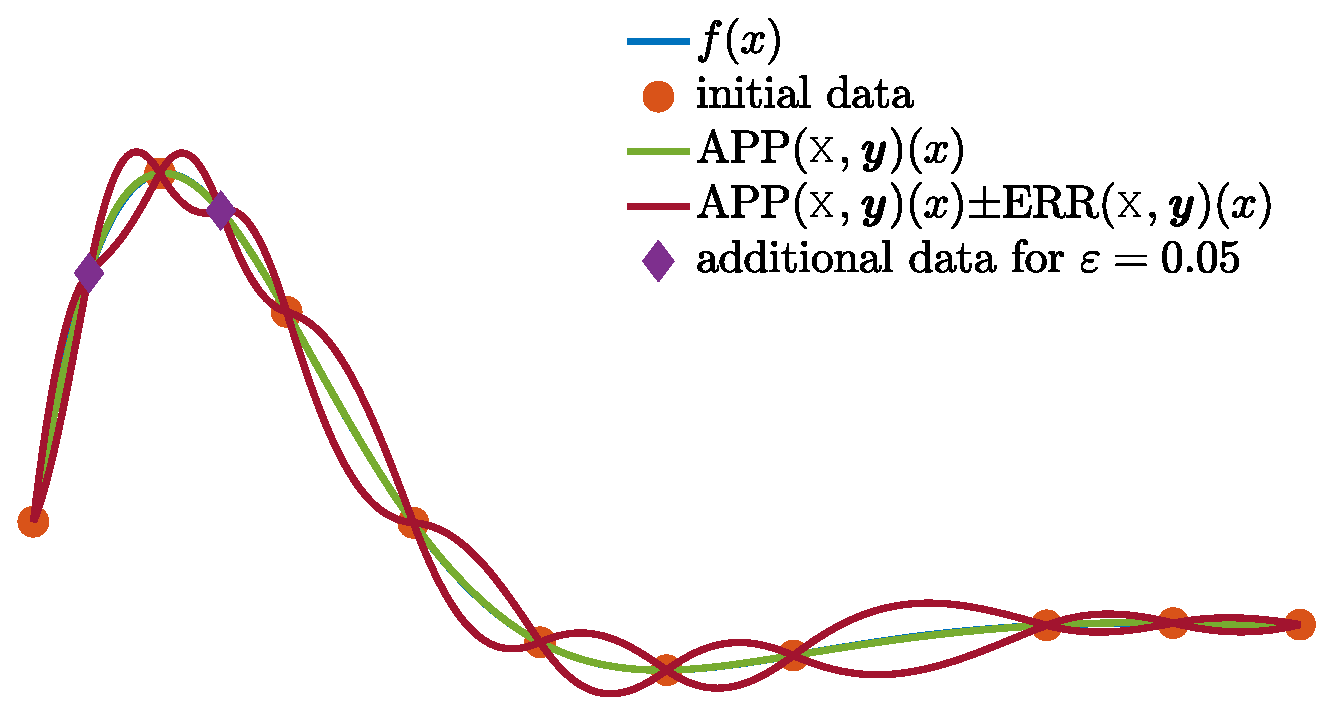
\includegraphics[width=6cm]{ProgramsImages/fandDataAndAppxAndRMSPEOptyFinal50.eps}}\vspace{-5ex}}
		\only<5>{\northeaststuff{3.5}{2.45}{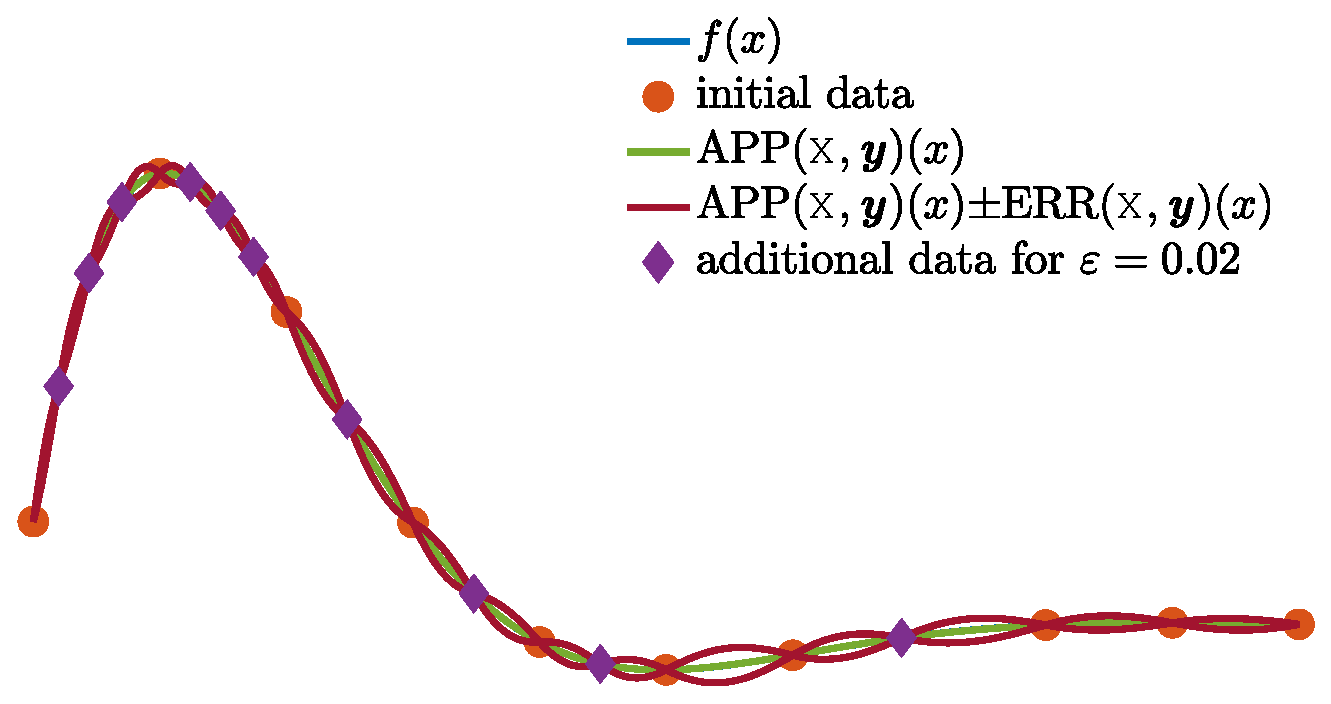
\includegraphics[width=6cm]{ProgramsImages/fandDataAndAppxAndRMSPEOptyFinal20.eps}}\vspace{-5ex}}
	
	
	\begin{minipage}{8cm}
		$\cf_{\vtheta}$ is a \alert{Hilbert space }  with \alert{reproducing kernel} $K_{\vtheta}$
		
		\vspace{-3ex}
		\begin{align*}
		\cc & =  \bigl\{ f \in \mathop{\cup} _{\vtheta} \, \cf_{\vtheta} :  \norm[\cf_{\vtheta^*}]{f - \app(\mX,\vy)} \le  \alert{\fC(\mX)} \norm[\cf_{\vtheta^*}]{f} \\
		&\qquad \qquad \forall \mX, \ \vy = f(\mX), \ \vtheta^*(\mX,\vy) \text{ given below} \bigr\} \\
		\only<1-2>{\text{e.g., } & K_{\vtheta}(\vt,\vx) = (1 + \norm[2]{\vtheta \odot(\vt - \vx)}) \exp\bigl( -\norm[2] {\vtheta \odot(\vt - \vx)}\bigr)}
		\only<3->{\text{e.g., } &  K_{\vtheta}(\vt,\vx) = \exp(\vb^T(\vt+\vx)) \\
			& \qquad \times (1 + \norm[2]{\va \odot(\vt - \vx)}) \exp\bigl( -\norm[2] {\va \odot(\vt - \vx)}\bigr) , \ 
		\vtheta  =(\va,\vb)}
		\end{align*}
	\end{minipage}
	
	\vspace{-2ex}\only<2>{\vspace{2ex}}
		Choose the $\vtheta$ (inspired by empirical Bayes) \alert{by minimizing the ellipsoid in $\reals^n$ of function data yielding interpolants with no greater norm than that observed:}

	\vspace{-6ex}		
	\begin{align*}
\vtheta^* &= \argmin_\vtheta \left[\frac 1n \log \bigl( \det(\mK_\vtheta) \bigr) + \log \bigl ( \vy^T \mK_\vtheta^{-1} \vy \bigr)\right]
	\\
	\norm[\infty]{f - \app(\mX,\vy)}^2 
	& \le \bignorm[\infty]{K(\cdot,\cdot) -  K(\cdot,\mX)\bigl(K(\mX,\mX) \bigr)^{-1} K(\mX, \cdot)} \ \frac{\fC^2(\mX)}{1 - \fC^2(\mX)} \ \vy^T(K(\mX,\mX) )^{-1} \vy =: \alert{\ERR^2(\mX,\vy)} \\
	\ACQ(\vx,\mX,\vy)  & : = \bigl[K(\vx,\vx) -  K(\vx,\mX)\bigl(K(\mX,\mX) \bigr)^{-1} K(\mX, \vx) \bigr]  \ \frac{\fC^2(\mX)}{1 - \fC^2(\mX)}  \ \vy^T(K(\mX,\mX) )^{-1} \vy \\[-1ex]
	\vx_{n+1} &= \argmax_{\vx \in \cx} \ACQ(\vx,\mX,\vy) \text{ \alert{acquisition function}}
	\end{align*}
	
\end{frame}


\begin{frame}
	{Cheng and Sandu Function\footfullcite{BinSur13, ChenSan10a}}
	\begin{tabular}{p{0.32\textwidth}@{\;}p{0.32\textwidth}@{\;}p{0.32\textwidth}}
		\multicolumn{1}{>{\centering}p{0.32\textwidth}}{$f(\vx) = \cos(x_1 + x_2) \exp(x_1 x_2)$} &
		\multicolumn{1}{>{\centering}p{0.32\textwidth}}{error w/ Mat\'ern \&  $\vtheta = \vone$} & \multicolumn{1}{>{\centering}p{0.32\textwidth}}{
		error w/ mod.\ Mat\'ern + opt.\ $\vtheta$ \newline $\varepsilon = 0.05$}
		\tabularnewline
		\hspace{-0.75cm}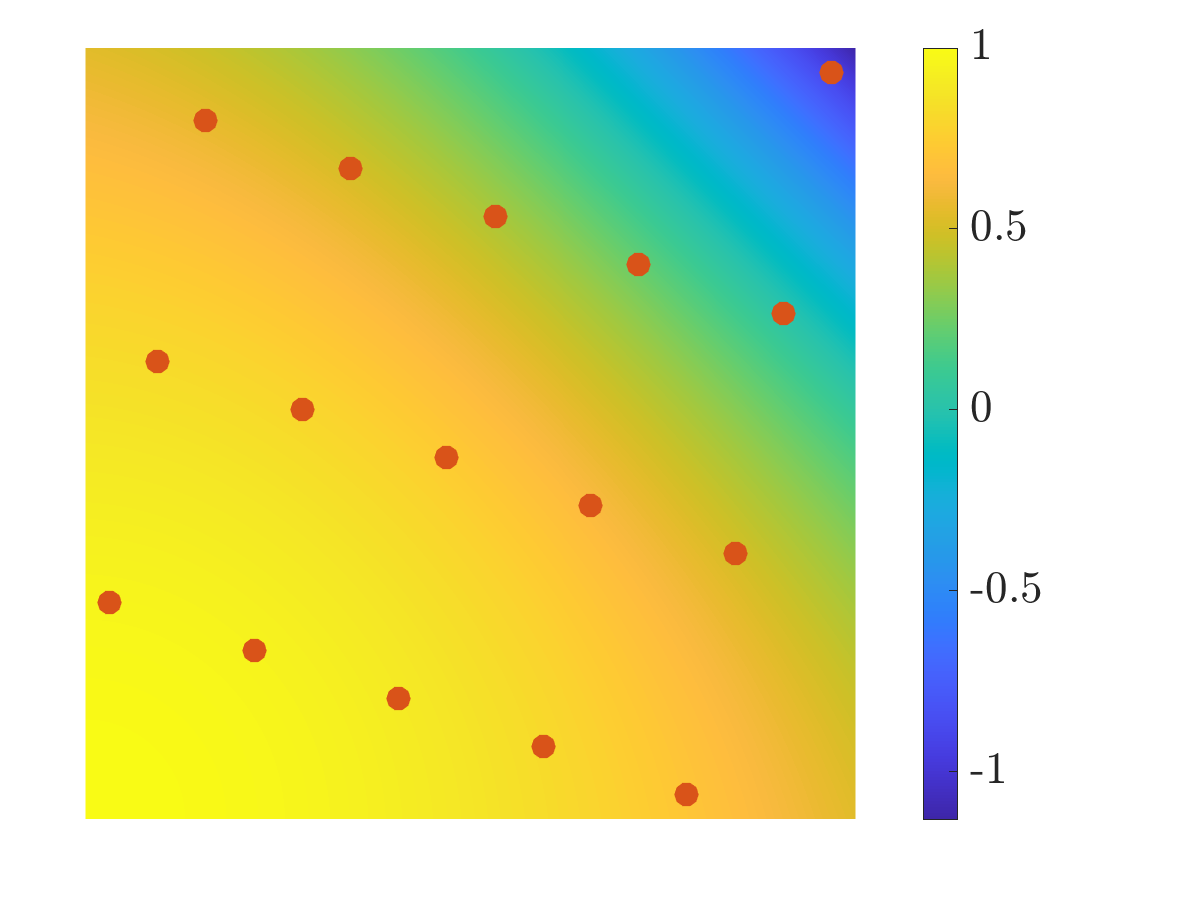
\includegraphics[width = 0.4\textwidth]{ProgramsImages/ChengFunData.eps}
		&
		\hspace{-0.6cm}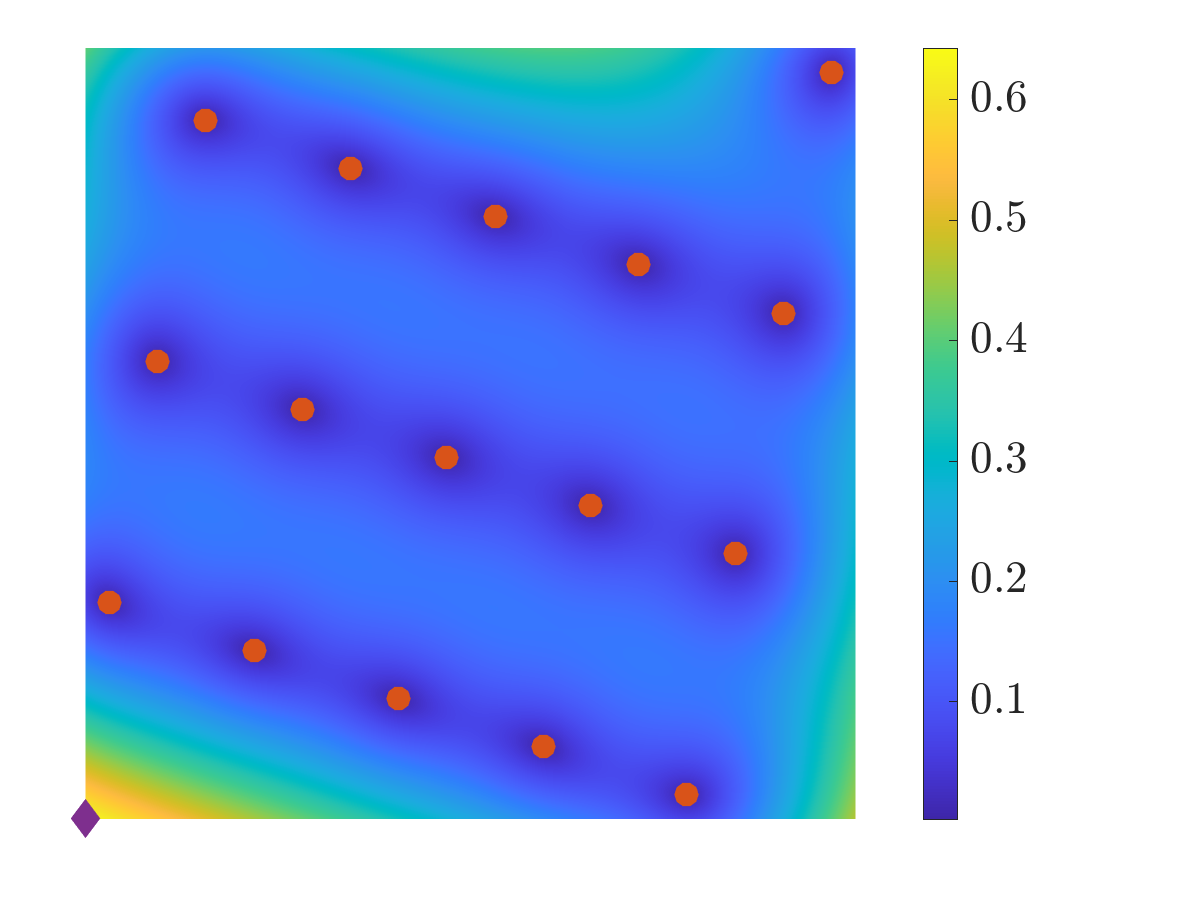
\includegraphics[width = 0.4\textwidth]{ProgramsImages/ChengFunErrNoOpt.eps}
&
		\only<1>{\hspace{-0.45cm}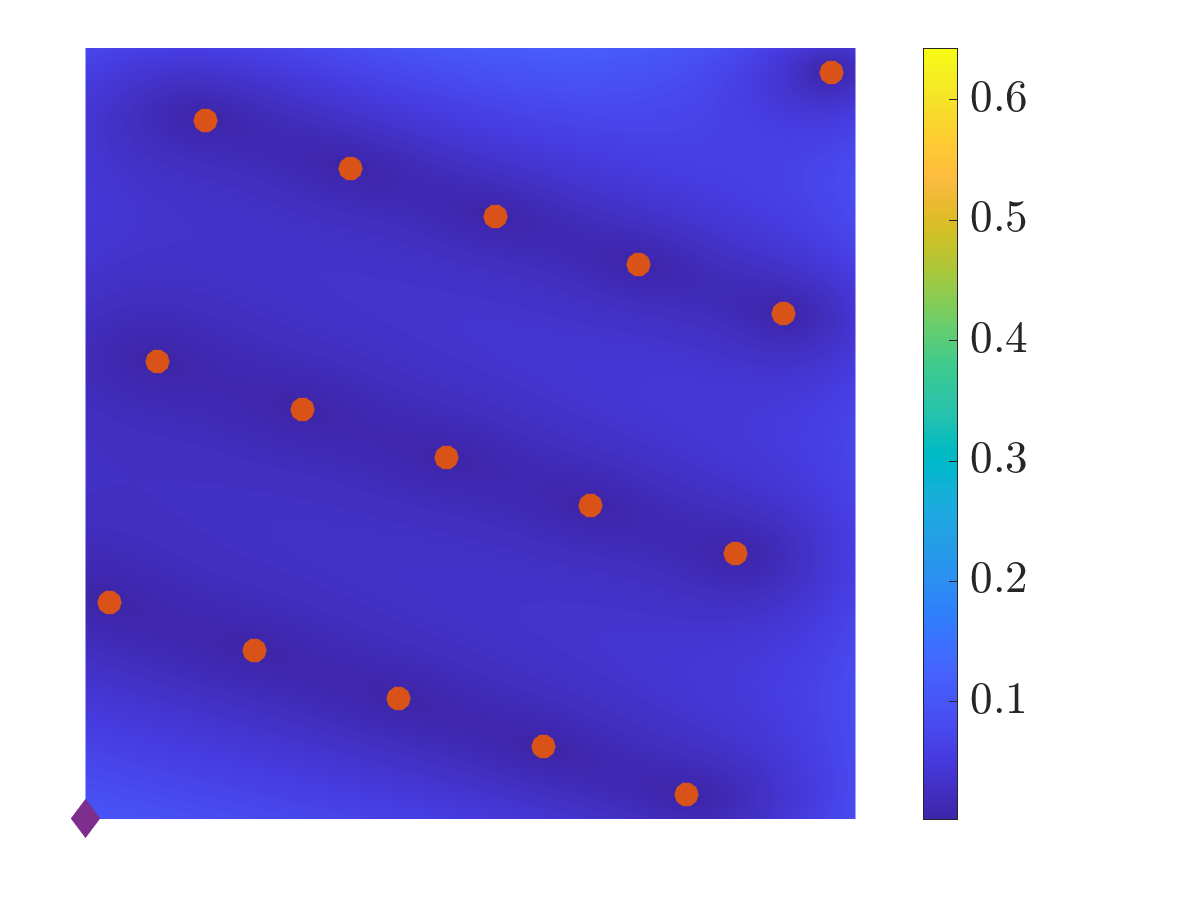
\includegraphics[width = 0.4\textwidth]{ProgramsImages/ChengFunErrOpty.eps}}
		\only<2>{\hspace{-0.45cm}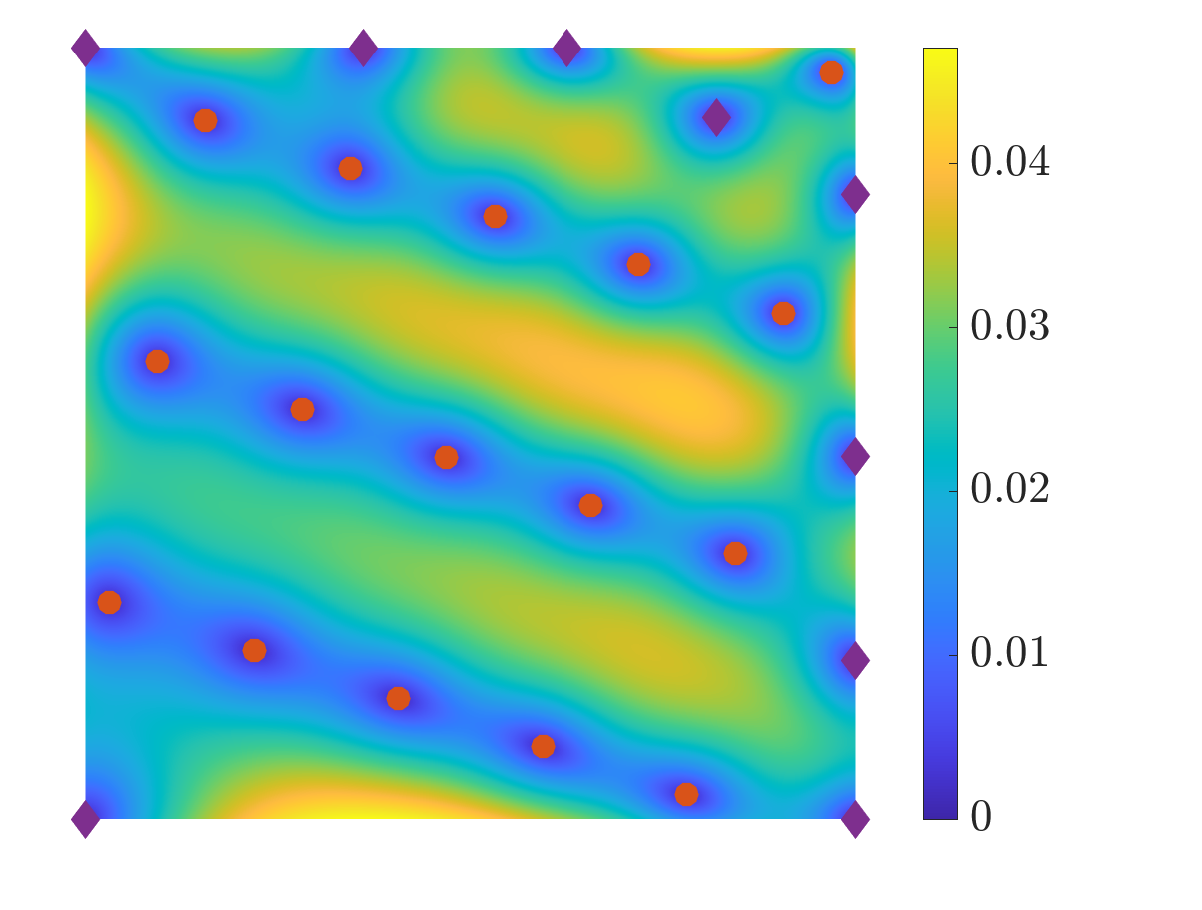
\includegraphics[width = 0.4\textwidth]{ProgramsImages/ChengFunErrOptyFinal.eps}}
	\end{tabular}
\end{frame}


\section{Summary}

\vspace{-6ex}

\begin{frame}
	{What Are the Right Ingredients for Adaptive Function Approximation?}
	
	\begin{itemize}
		\item A fixed budget \alert{homogeneous approximation}, $\app : \cx^n \times \reals^n \to L^{\infty}(\cx)$, with an error bound, e.g., linear splines, RKHS approximation
		
		\item An unbounded, non-convex \alert{candidate set}, $\cc$, for which the error bound can be bounded in \alert{data-driven} way; what you see is almost what you get
		
		\item \alert{Necessary} conditions for $f$ to lie in $\cc$; will not have sufficient conditions
		
		\item A rich enough candidate set from which the right approximation can be \alert{inferred}; attention to underfitting and overfitting
		
			
	\end{itemize}


	\uncover<2->{
	\begin{itemize}
	\item More work is needed on 
	
	\begin{itemize}
		
		\item What makes a good initial sample
	
		\item Balancing the richness of the candidate set with overfitting
		
		\item Numerical instability and computational effort challenges for larger numbers of data sites. 
	
	
\end{itemize}
\end{itemize}
}


\end{frame}



\finalthanksnote{These slides are  available at \\  \href{https://speakerdeck.com/fjhickernell/right-ingredients-for-adaptive-function-approximation}{\nolinkurl{speakerdeck.com/fjhickernell/right-ingredients-for-adaptive-function-approximation}}}


\thankyouframe


\begin{frame}
	\frametitle{References}
\printbibliography
\end{frame}




\end{document}

\begin{frame}{What Should $\fC(\mX)$ Be?}
	\[
	\cc  =  \bigl\{ f \in \cf :  \norm[\cf]{f - \app(\mX,\vy)} \le  \alert{\fC(\mX)} \norm[\cf]{f} \bigr\}
	\]
	As $\mX$ covers $\cx$ better, $\fC(\mX)$ should decrease.  Suggest choosing
	\begin{align*}
	\frac{ \norm[\cf]{f - \app(\mX,\vy)}^2 }{ \norm[\cf]{f}^2 } = \fC^2(\mX) & : = \fC_0^2 \norm[\infty]{\frac{\sup \{ \abs{f(\cdot)}^2 : \norm[\cf]{f} \le 1,   \ f(\mX) = \vzero  \}}{\sup \{ \abs{f(\cdot)}^2 : \norm[\cf]{f} \le 1 \}}} \\
	&  = \fC_0^2  \norm[\infty]{\frac{K(\cdot,\cdot) -  K(\cdot,\mX)\bigl(K(\mX,\mX) \bigr)^{-1} K(\mX, \cdot)}{K(\cdot,\cdot)}}
	\end{align*}
	
	
\end{frame}


